
\documentclass[fleqn,addpoints]{exam}

\usepackage{amsmath}
\usepackage{mdwlist}
% \usepackage{graphics}
\usepackage{graphicx}
\usepackage{cancel}
% \usepackage{polynom}
\usepackage{float}

% \printanswers

\ifprintanswers
\usepackage{2in1, lscape}
\fi

\title{Math 113 Homework 18}
\author{}
\date{\today}

\begin{document}

\maketitle

\section{From the Book}

\begin{itemize*}
  \item pp. 348-349: 1-3, 10-16, 26, 30, 31, 44, 45, 47
  \item pp. 356-357: 15-19, 38
  \item pg. 364: 15-19
\end{itemize*}

% 130 points possible

\ifprintanswers

\section{Pages 348-349}

\begin{description}

\item[1]
\begin{description}
  \item[a] $(-3,-4)$ - III
  \item[b] $(5,-6)$ - IV
  \item[c] $(-6,8)$ - II
  \item[d] $(-1,-6)$ - III
  \item[e] $(4,10)$ - I
  \item[e] $(9,-1)$ - IV
\end{description}

\item[2]
\begin{description}
  \item[a] 0
  \item[b] 0
\end{description}

\item[3]
\begin{description}
  \item[a] I and III
  \item[b] II and IV
  \item[c] II and III
  \item[d] III and IV
\end{description}

\item[10]
\( x^2 + 2y = 4\)
\begin{description}
  \item[x axis] - no
  \item[y axis] - yes
  \item[origin] - no
\end{description}

\item[11]
\( -3x + 2y^2 = -4 \)
\begin{description}
  \item[x axis] - yes
  \item[y axis] - no
  \item[origin] - no
\end{description}

\item[12]
\( x = -y^2 + 5 \)
\begin{description}
  \item[x axis] - yes
  \item[y axis] - no
  \item[origin] - no
\end{description}

\item[13]
\( y = 4x^2 + 13 \)
\begin{description}
  \item[x axis] - no
  \item[y axis] - yes
  \item[origin] - no
\end{description}

\item[14]
\( xy = -6 \)
\begin{description}
  \item[x axis] - no
  \item[y axis] - no
  \item[origin] - yes
\end{description}

\item[15]
\( 2x^2y^2 = 5 \)
\begin{description}
  \item[x axis] - yes
  \item[y axis] - yes
  \item[origin] - yes
\end{description}

\item[16]
\( 2x^2 + 3y^2 = 9 \)
\begin{description}
  \item[x axis] - yes
  \item[y axis] - yes
  \item[origin] - yes
\end{description}

\item[26]
$y=3x-6$
\begin{figure}[H]
  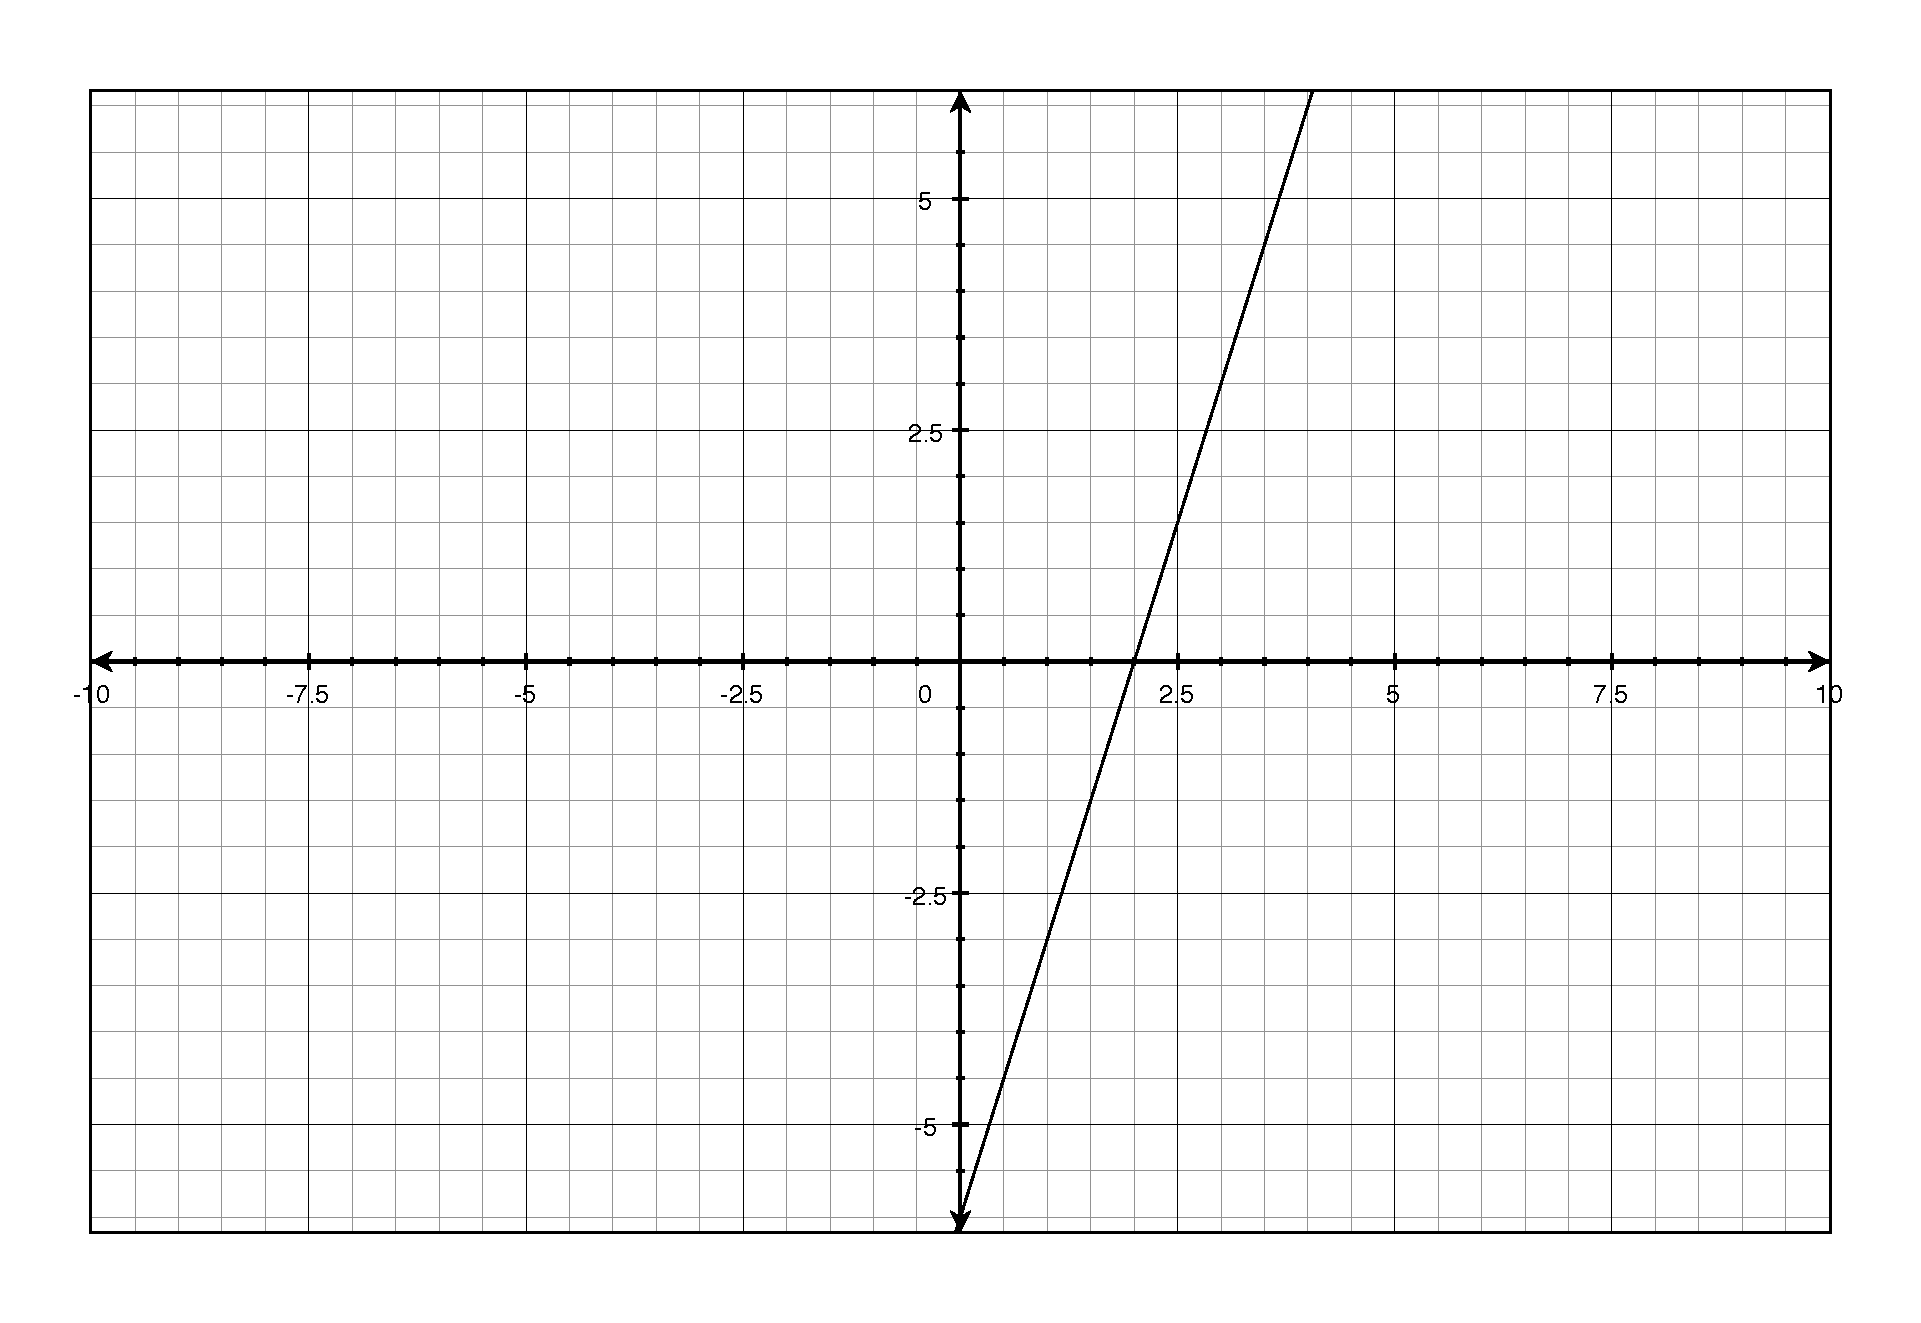
\includegraphics[width=9cm,height=7cm]{p318/26}
\end{figure}

\item[30]
$y=\dfrac{2}{3} x - 1$
\begin{figure}[H]
  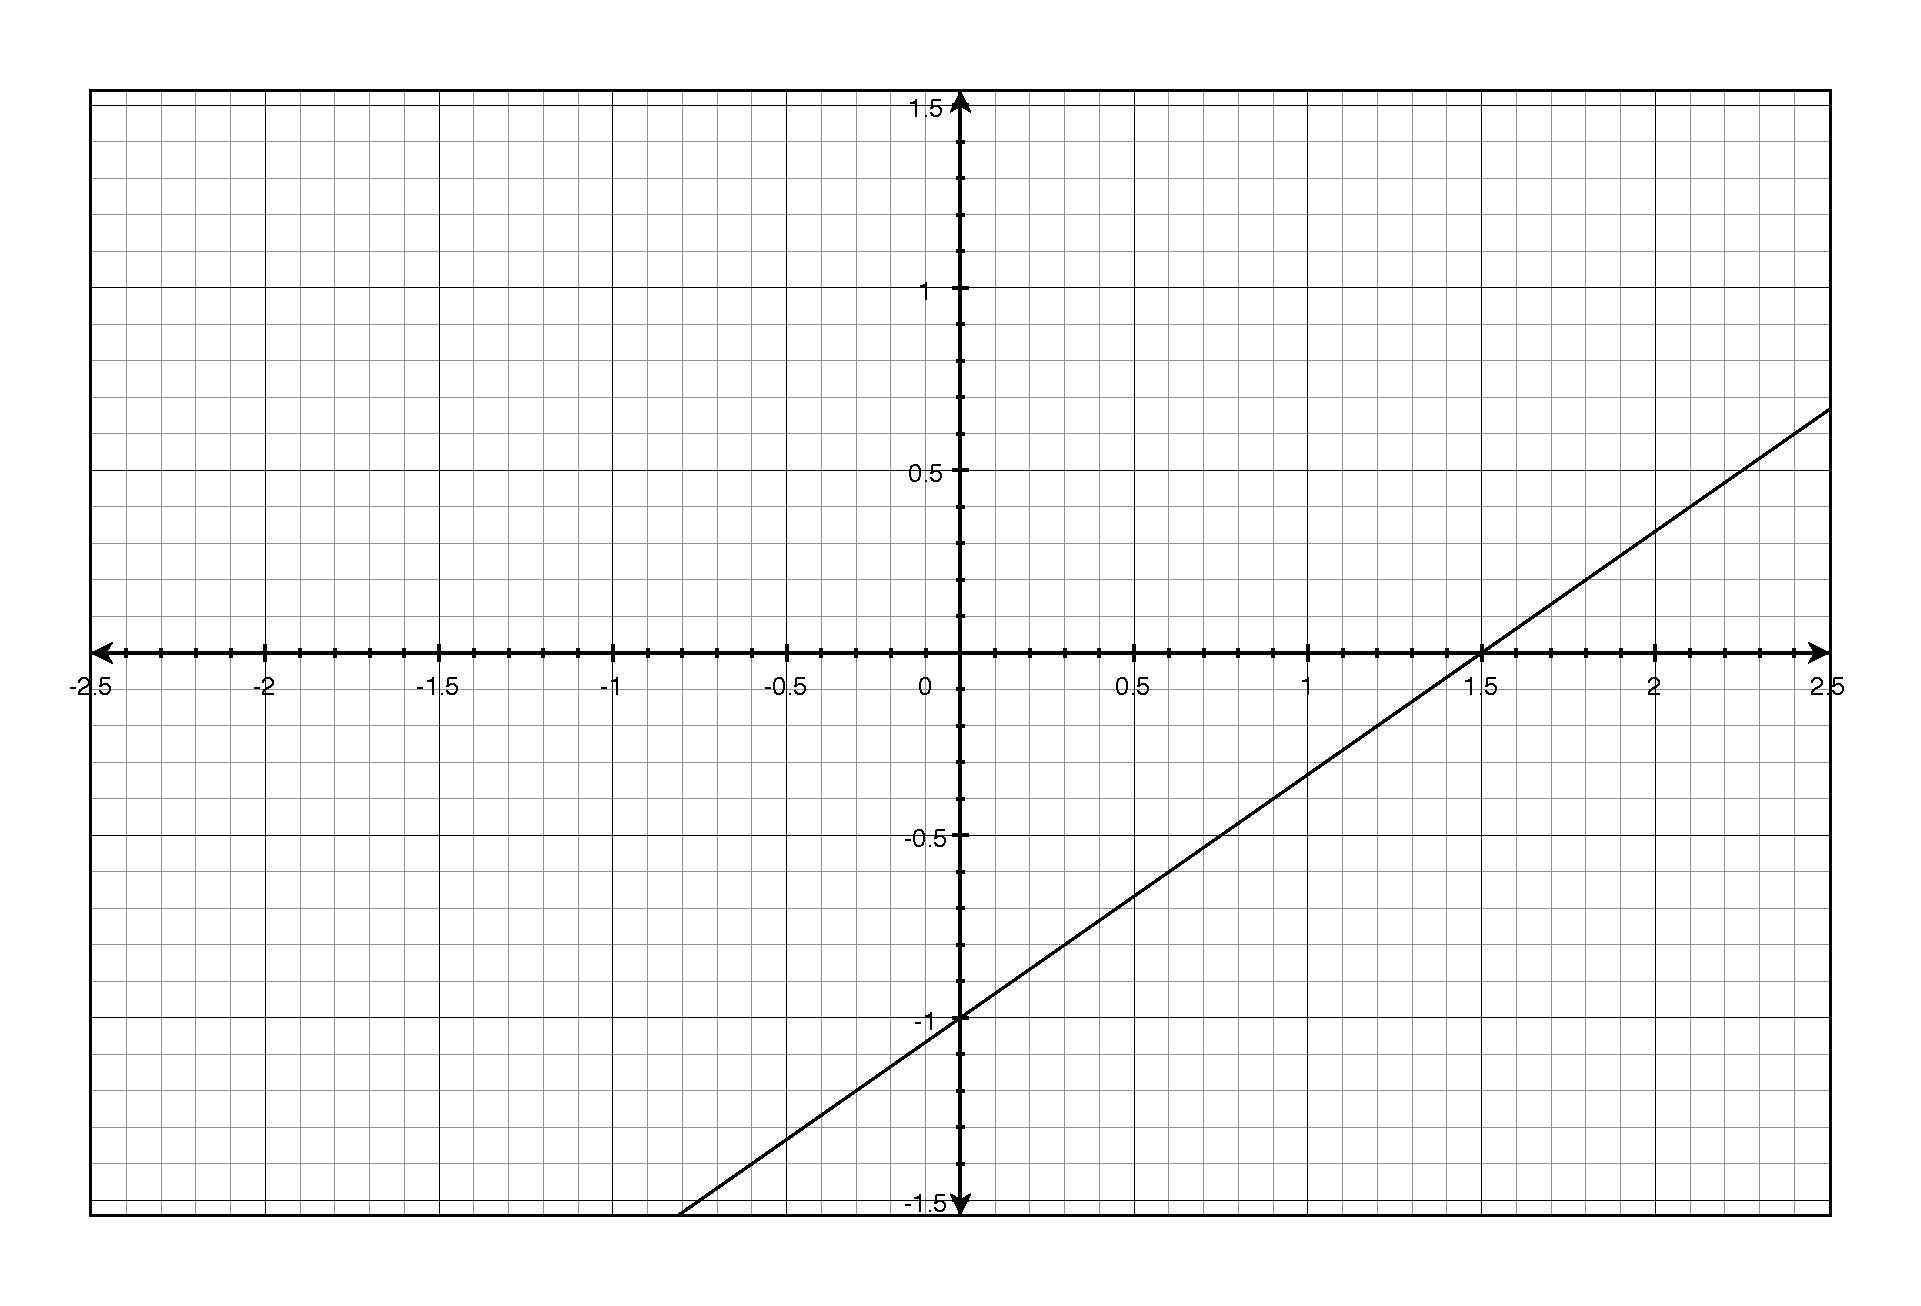
\includegraphics[width=9cm,height=7cm]{p318/30}
\end{figure}

\item[31]
$y= -\dfrac{1}{3} x + 2$
\begin{figure}[H]
  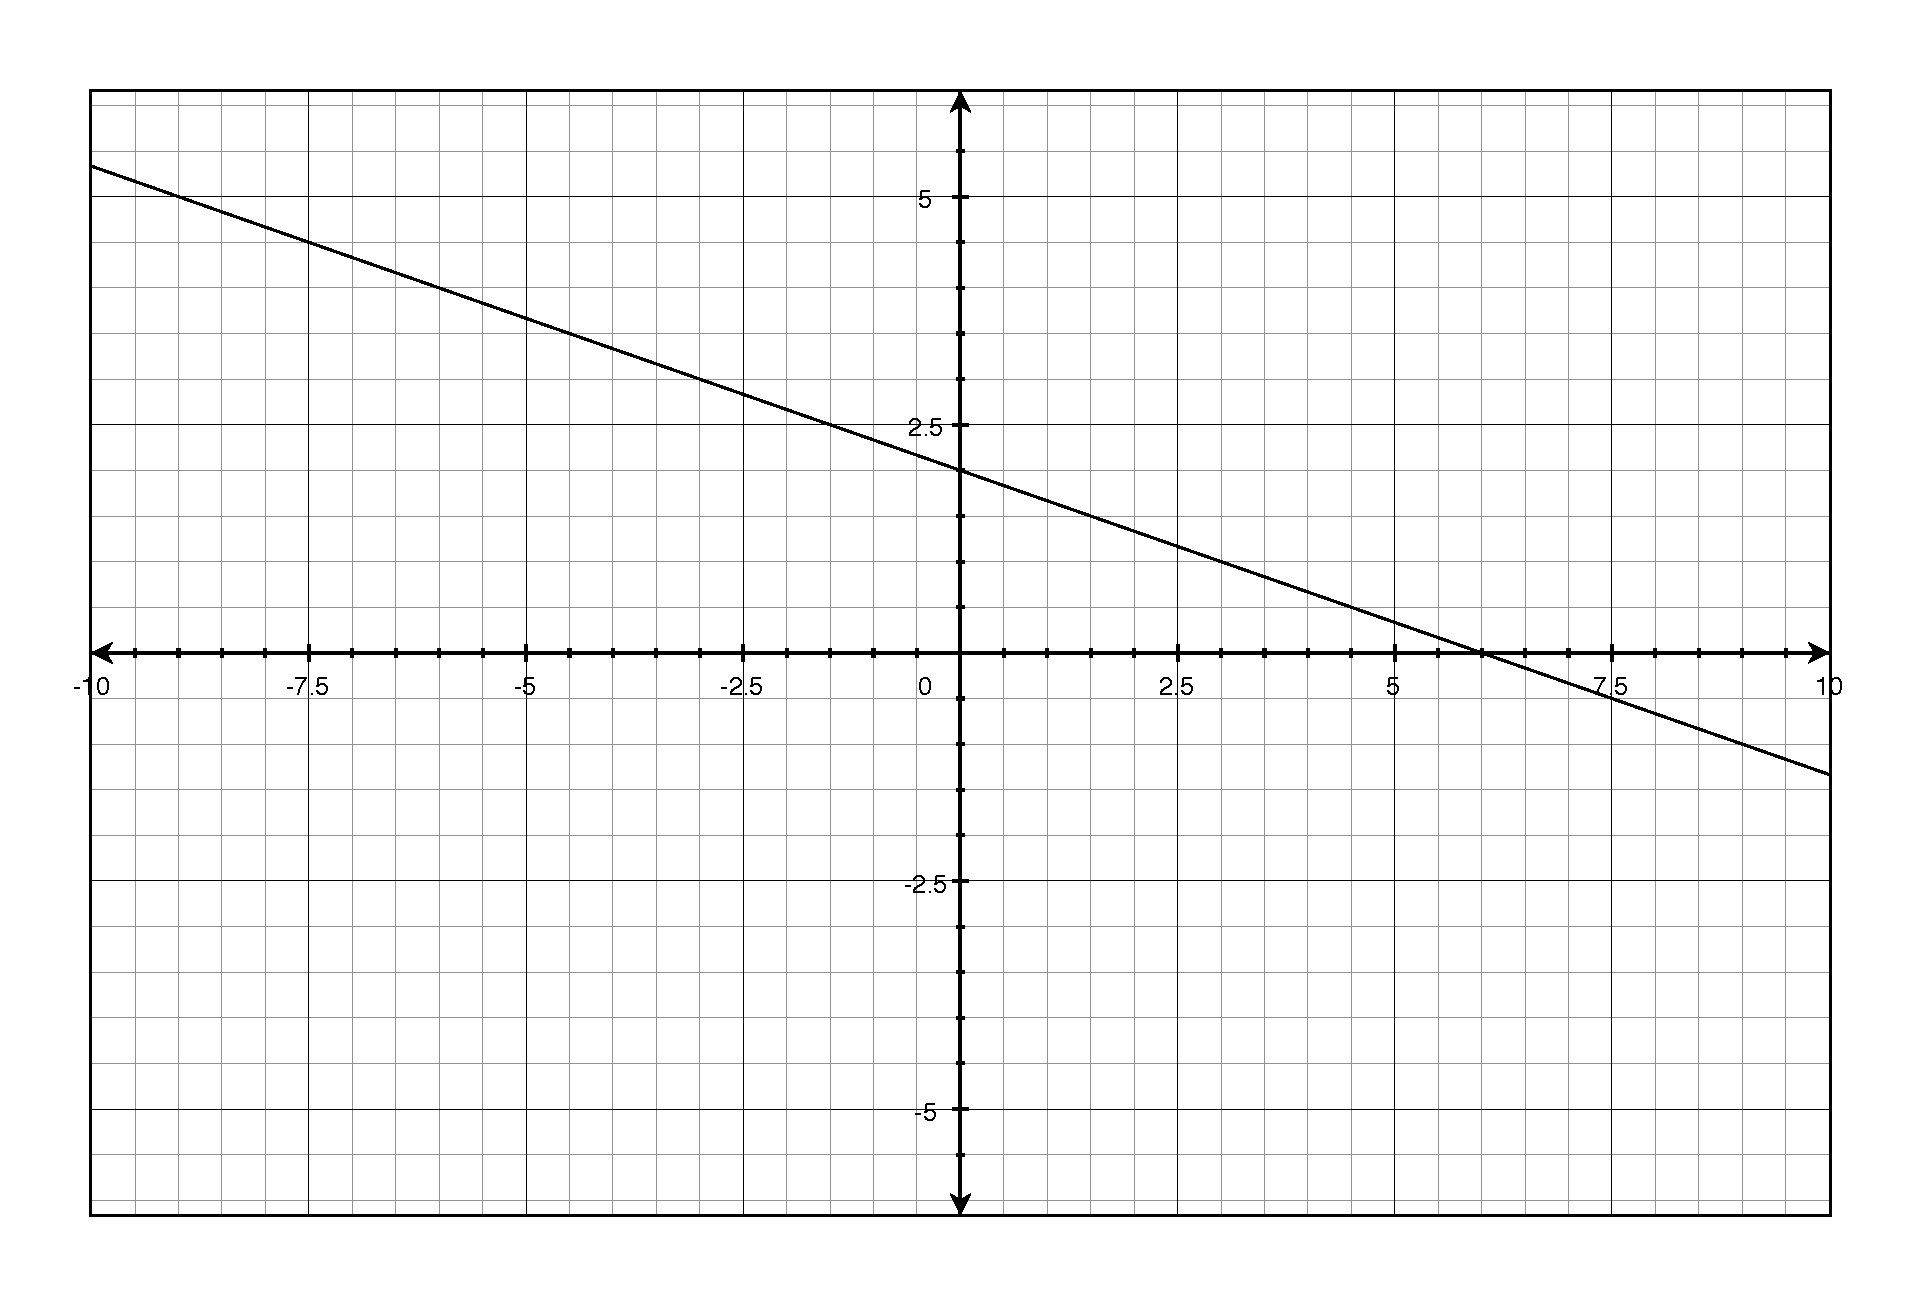
\includegraphics[width=9cm,height=7cm]{p318/31}
\end{figure}

\item[44]
$y= 2x^2$
\begin{figure}[H]
  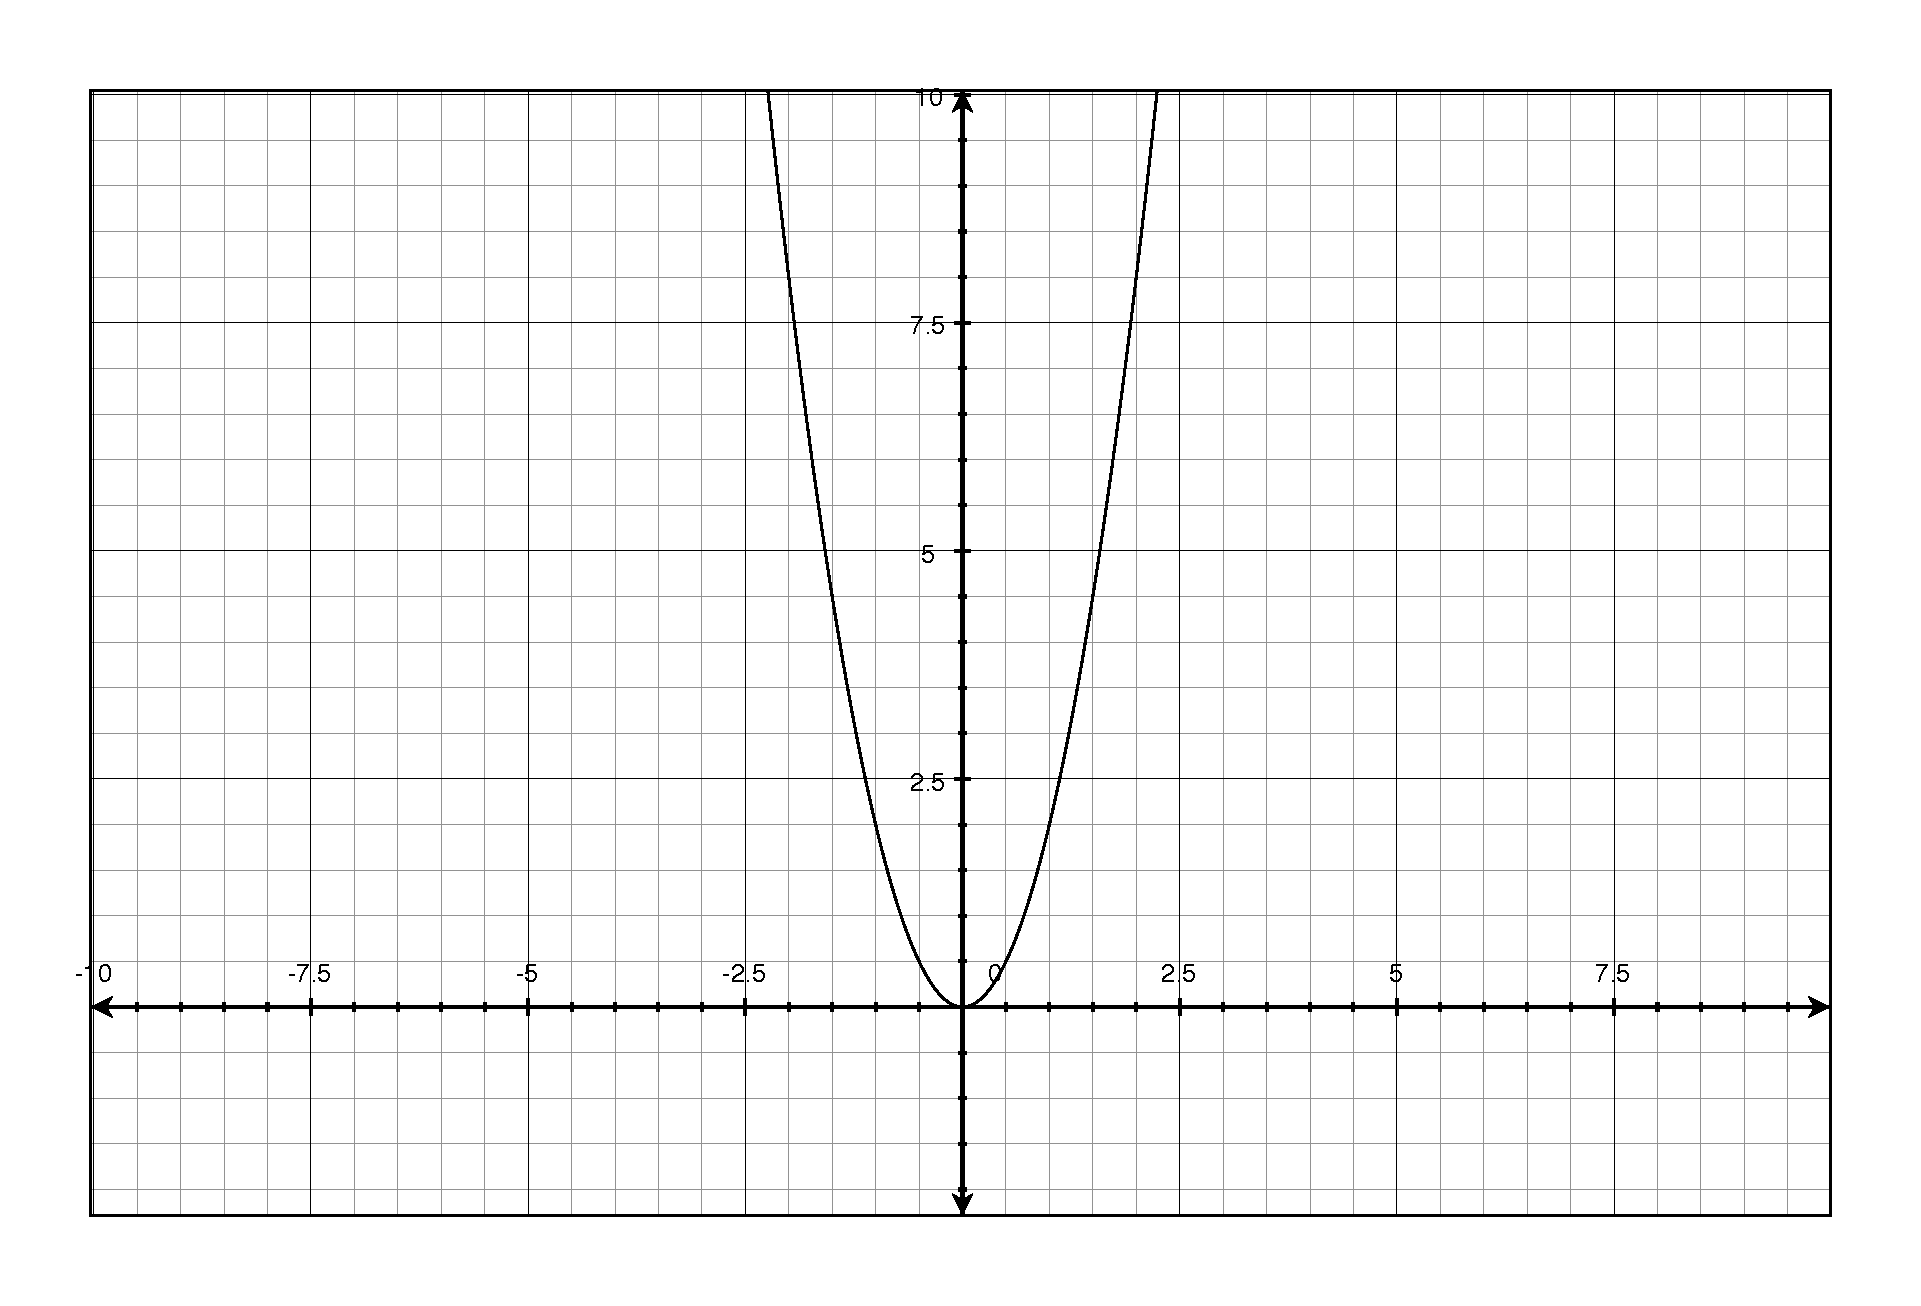
\includegraphics[width=9cm,height=7cm]{p318/44}
\end{figure}

\item[45]
$y= -3x^2$
\begin{figure}[H]
  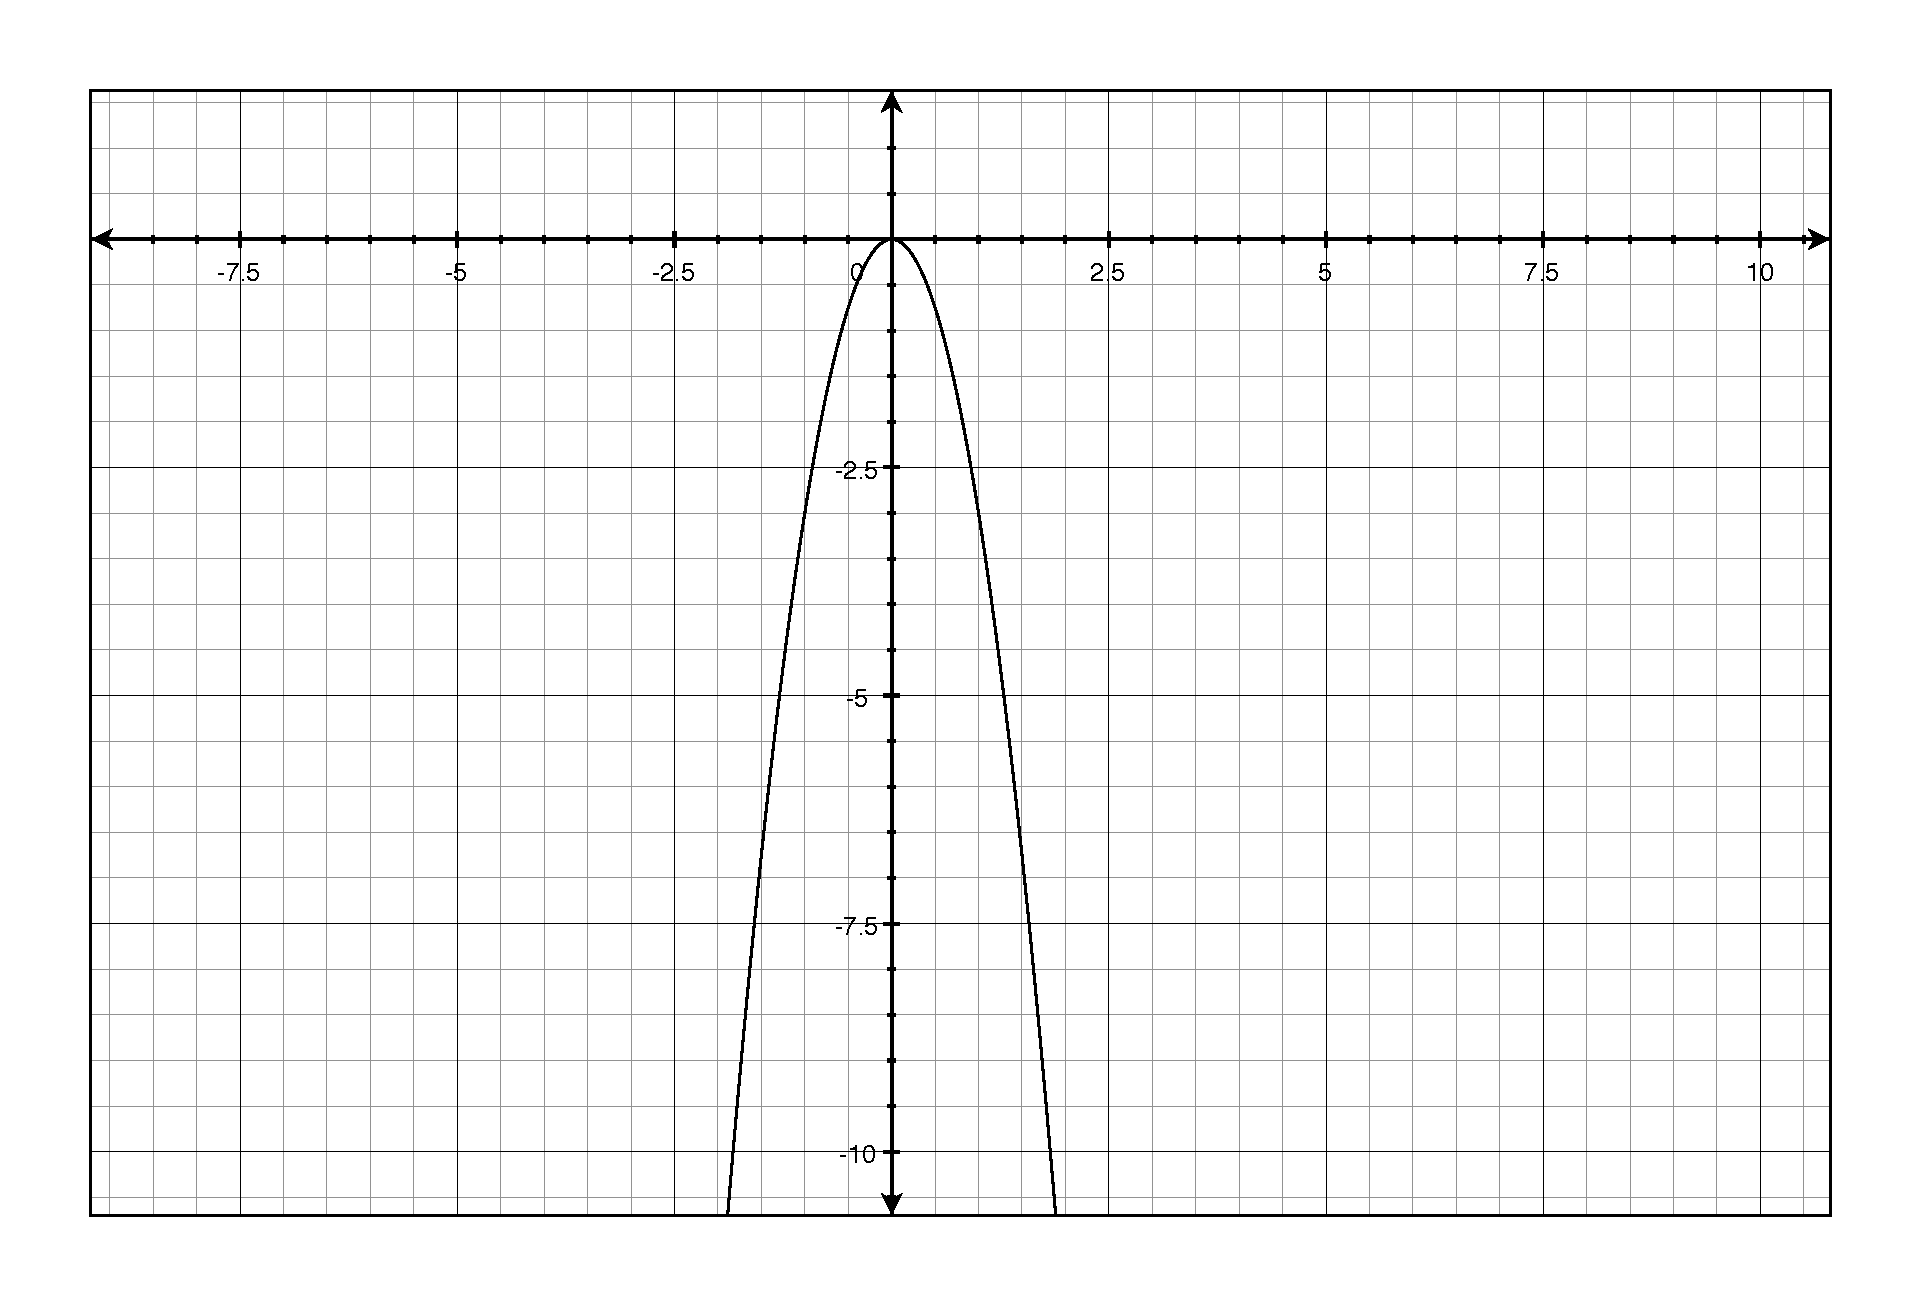
\includegraphics[width=9cm,height=7cm]{p318/45}
\end{figure}

\item[47]
$xy= 2$
\begin{figure}[H]
  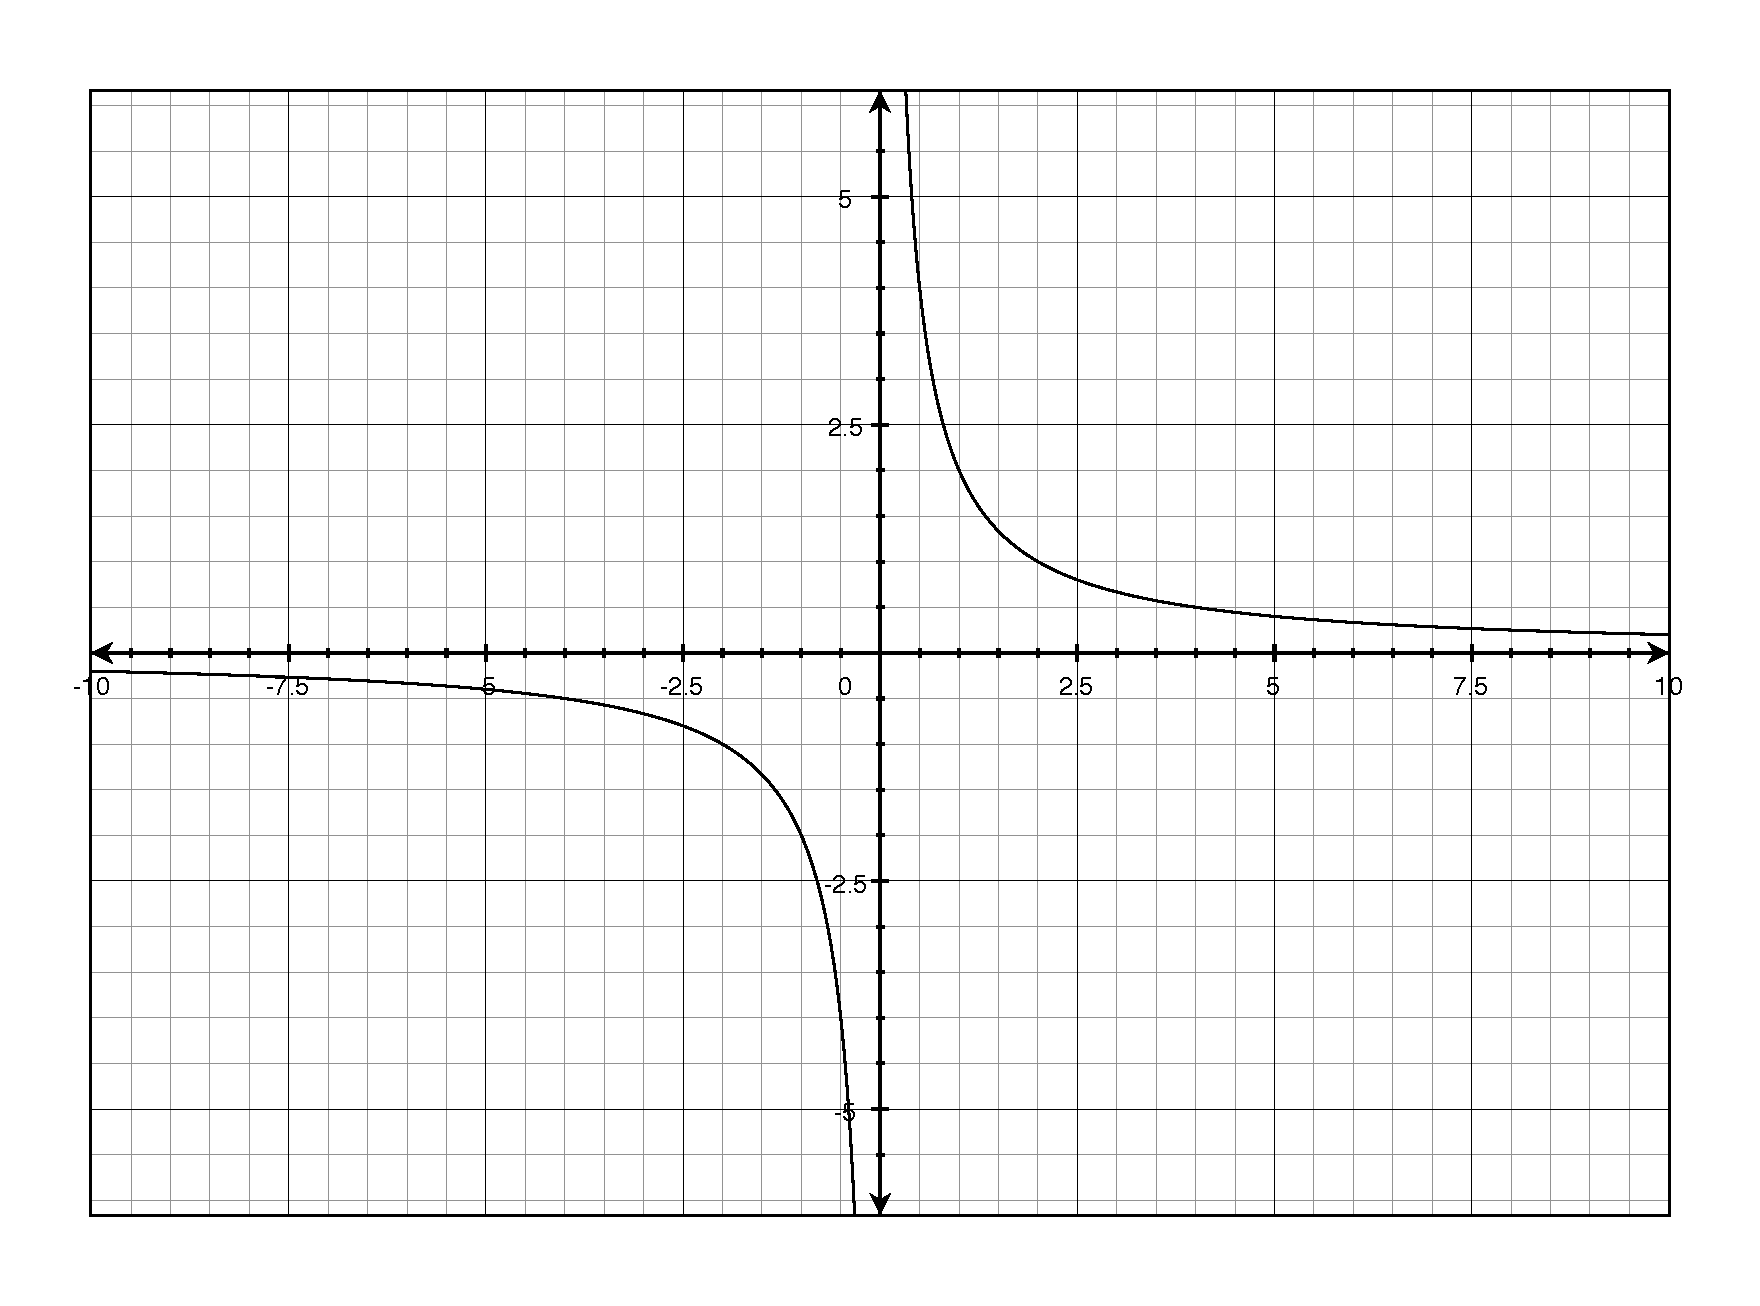
\includegraphics[width=9cm,height=7cm]{p318/47}
\end{figure}

\end{description}

\section{Pages 356-357}

\begin{description}

\item[15]
$y=-2x-1$
\begin{figure}[H]
  \includegraphics[width=9cm,height=7cm]{p356/15}
\end{figure}

\pagebreak

\item[16]
$y=4x+3$
\begin{figure}[H]
  \includegraphics[width=9cm,height=7cm]{p356/16}
\end{figure}

\item[17]
$y=\dfrac{1}{2} x + \dfrac{2}{3}$
\begin{figure}[H]
  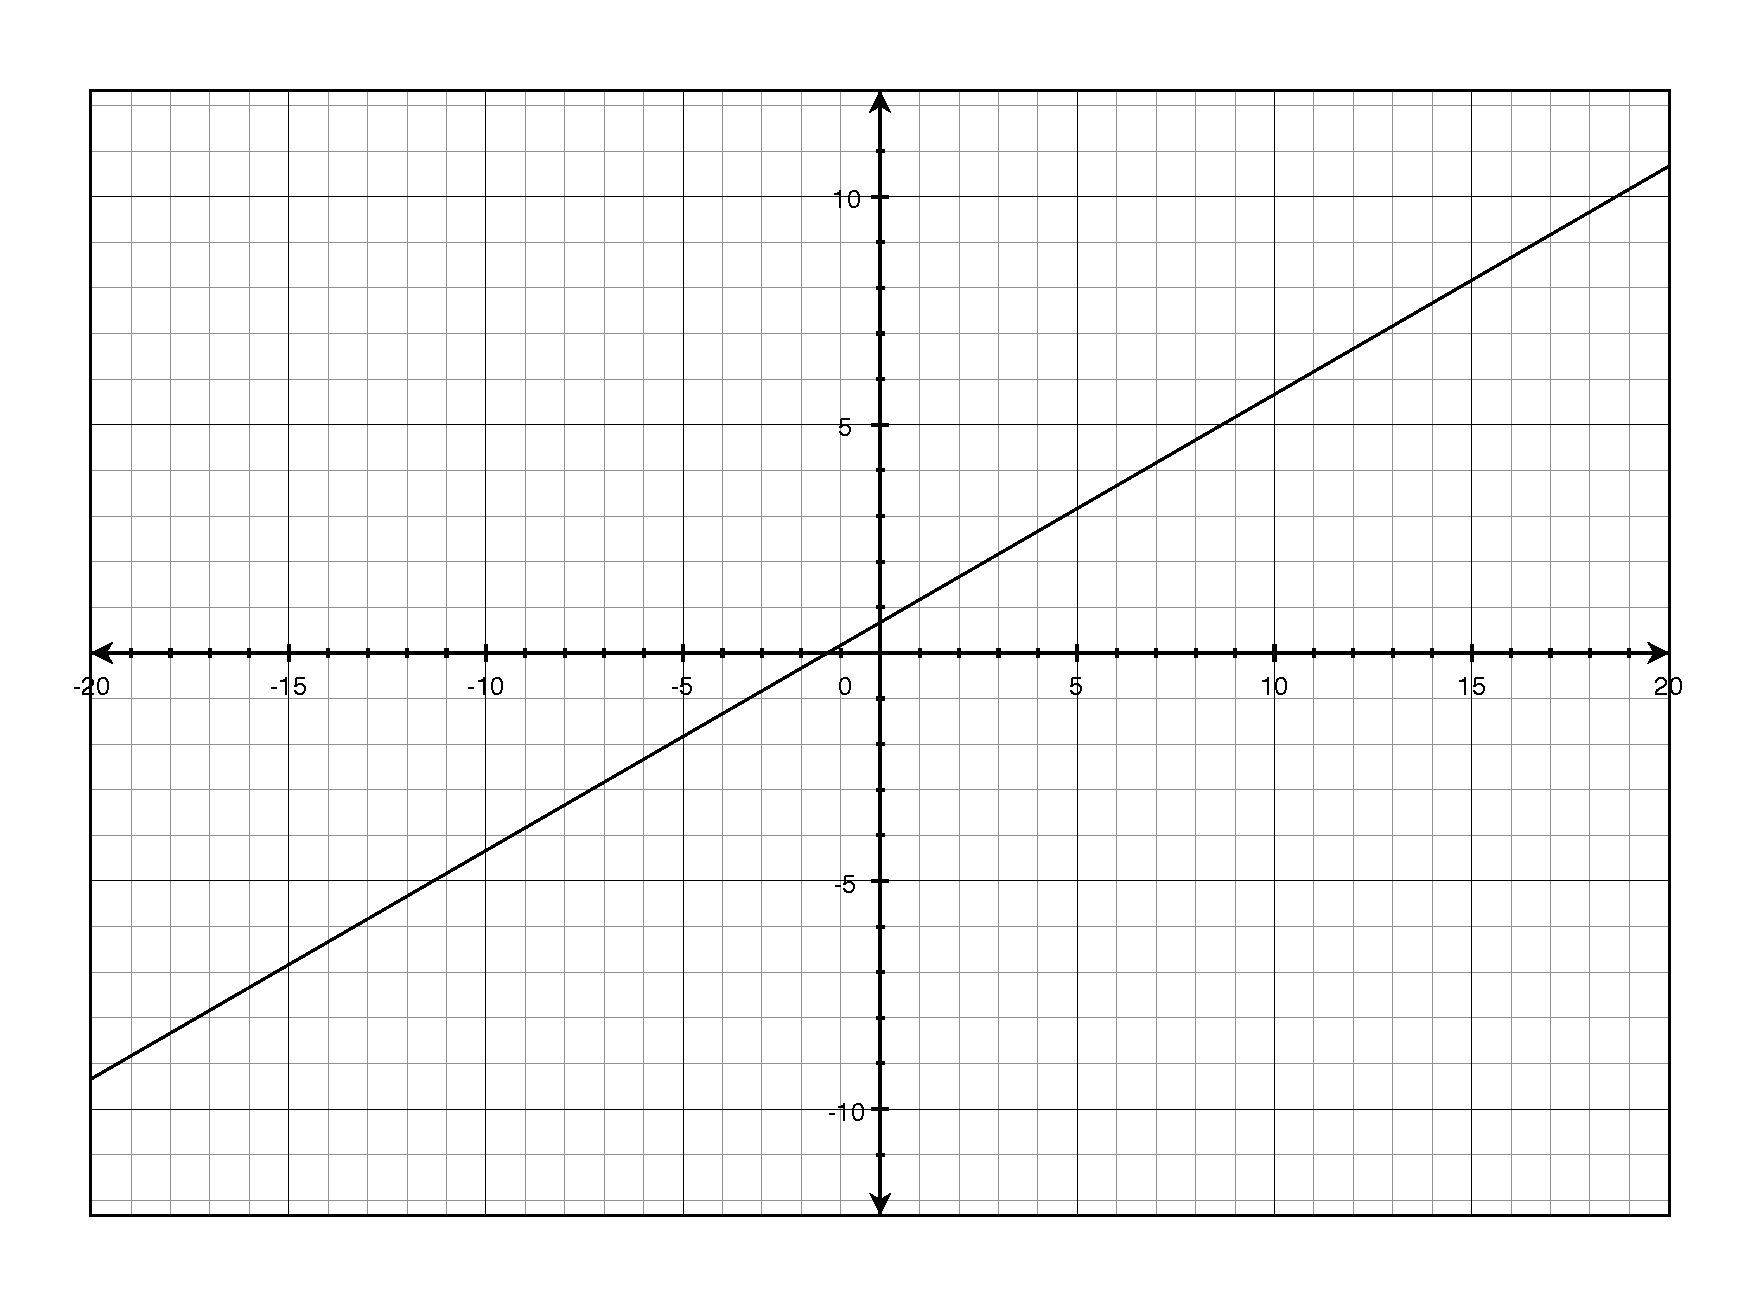
\includegraphics[width=9cm,height=7cm]{p356/17}
\end{figure}

\item[18]
$y= \dfrac{2}{3} x - \dfrac{3}{4}$
\begin{figure}[H]
  \includegraphics[width=9cm,height=7cm]{p356/18}
\end{figure}

\item[19]
$y=-x$
\begin{figure}[H]
  \includegraphics[width=9cm,height=7cm]{p356/19}
\end{figure}

\item[38]
\begin{description}
\item[a]
\begin{tabular}{| c | c |}
\hline
  C & F \\
\hline
\hline
  0 & 32 \\
  5 & 41 \\
  10 & 50 \\
  15 & 59 \\
  20 & 68 \\
  -5 & 23 \\
  -10 & 14 \\
  -15 & 5 \\
  -20 & -4 \\
  -25 & -13 \\
\hline
\end{tabular}

\item[b]
\begin{figure}[H]
  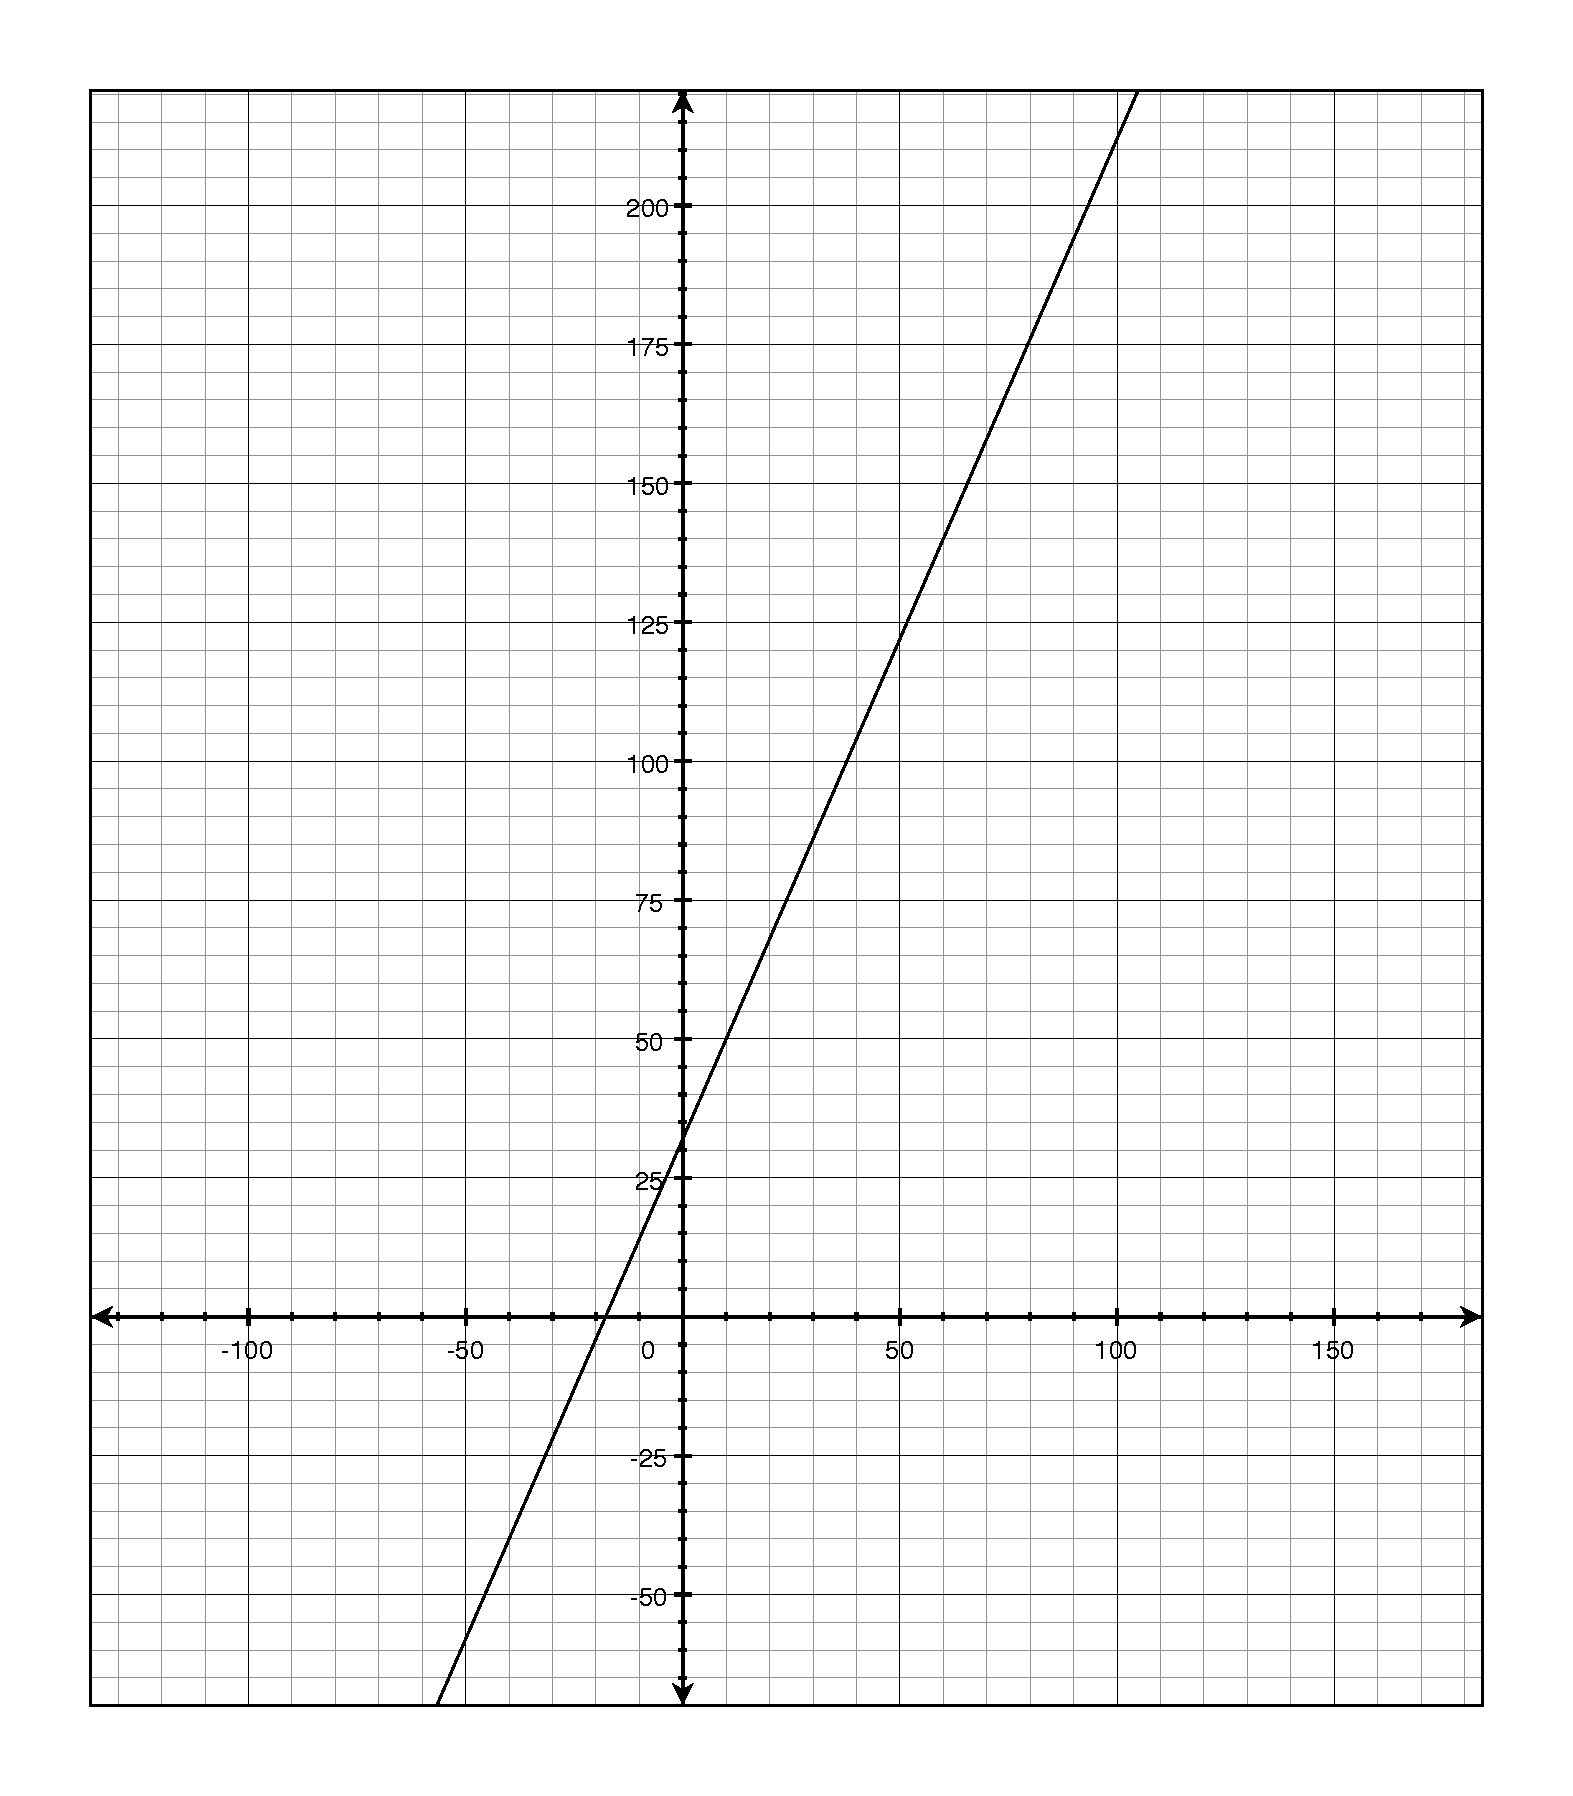
\includegraphics[width=9cm,height=7cm]{p356/38}
\end{figure}

\item[c]
\begin{tabular}{| c | c |}
\hline
  C & F \\
\hline
\hline
  25 & 77 \\
  30 & 86 \\
  -30 & -22 \\
  -40 & -40 \\
\hline
\end{tabular}

\end{description} % problem 38
\end{description} % section

\section{Page 364}

\begin{description}

\item[15]
$y > - \dfrac{3}{2} x - 3$
\begin{figure}[H]
  \includegraphics[width=9cm,height=7cm]{p364/15}
\end{figure}

\pagebreak

\item[16]
$2x+5y > -4$
\begin{figure}[H]
  \includegraphics[width=9cm,height=7cm]{p364/16.eps}
\end{figure}

\item[17]
$y < - \dfrac{1}{2} x + 2$
\begin{figure}[H]
  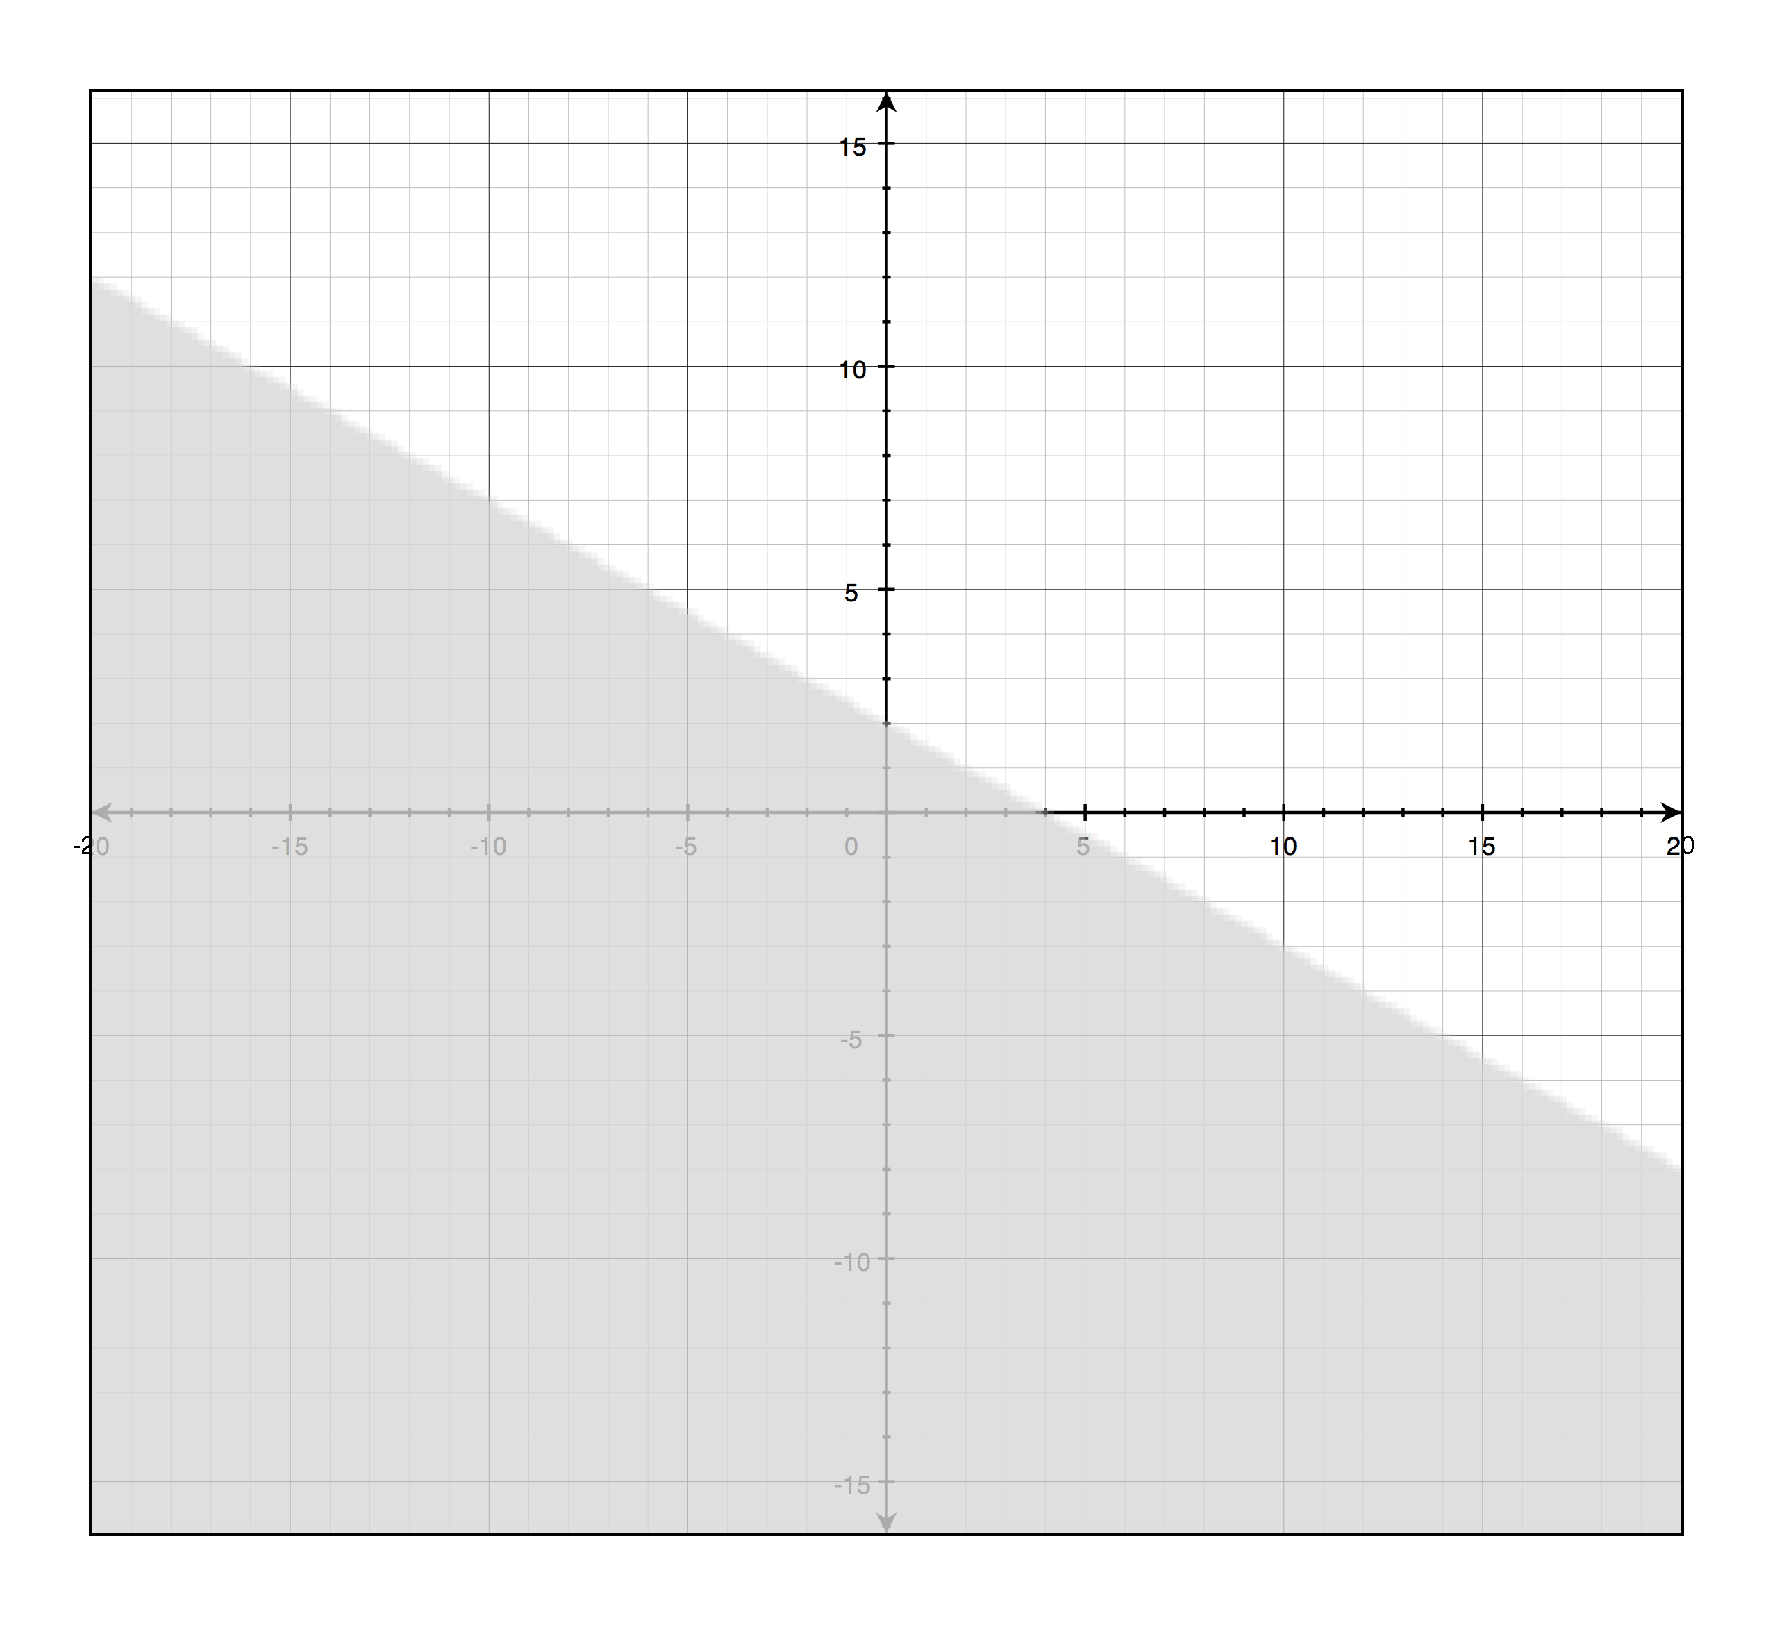
\includegraphics[width=9cm,height=7cm]{p364/17}
\end{figure}

\pagebreak

\item[18]
$y < - \dfrac{1}{3} x + 1$
\begin{figure}[H]
  \includegraphics[width=9cm,height=7cm]{p364/18}
\end{figure}

\item[19]
$x \leq 3$
\begin{figure}[H]
  \includegraphics[width=9cm,height=7cm]{p364/19}
\end{figure}

\end{description}

\fi

\section{Extra Credit}

Find the length of side $a$ in the following figure:

\begin{figure}[H]
  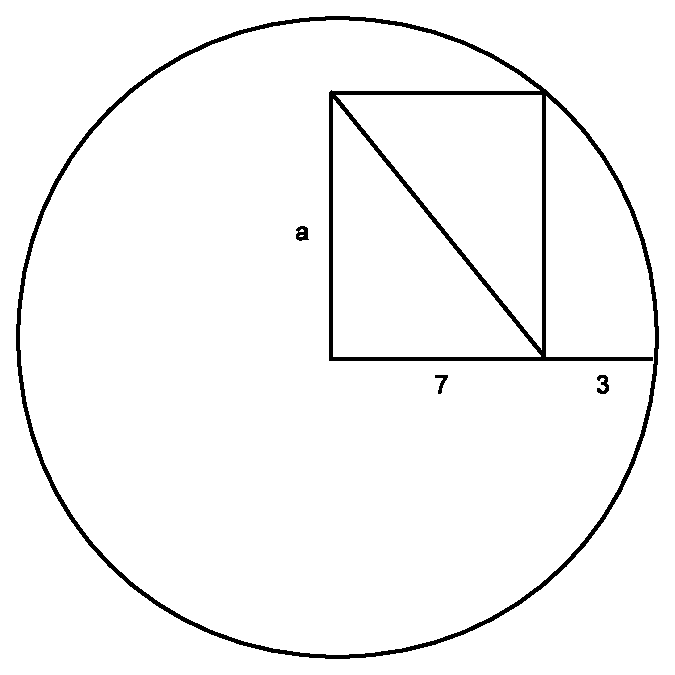
\includegraphics[width=6cm]{extra-credit}
\end{figure}
\label{extra-credit}

\ifprintanswers

If you draw the other diagonal in the rectangle, you can see that the diagonal is the radius of the circle.  The radius
is $7+3=10$.  So you have a right triangle with a hypotenuse of $10$ and one side equal to $7$.  You can use the
Pythagorean theorem to find the other side:

\begin{align*}
  a^2 + 7^2 &= 10^2 \\
  a^2 + 49 &= 100 \\
  a^2 &= 51 \\
  a &= \sqrt{51}    
\end{align*}

\else
\vspace{1.5 in}

\begin{em}
You're not supposed to be so blind with patriotism that you can't face reality. Wrong is wrong no matter who does it or who says it. 
\end{em}

\vspace{0.1 in}
\hspace{0.5 in} --Malcolm X

\fi

\end{document}

